
\chapter{Monte Carlo simulation}\label{chap:MC}
\minitoc
The Monte Carlo (MC) method was invented by scientists working on the atomic bomb in the 1940s. Its core idea is to use random samples of parameters or inputs to explore the behavior of a complex system or process.  Nowadays, MC simulation is the  essential part of research in both theoretical and experimental particle physics.
This chapter gives an overview of the ATLAS experiment simulation scheme, the simulation methods and the simulation software. Moreover, techniques for fast simulation are discussed. 

\section{Monte Carlo production in \atlas}

\begin{figure}[!b]
\center{
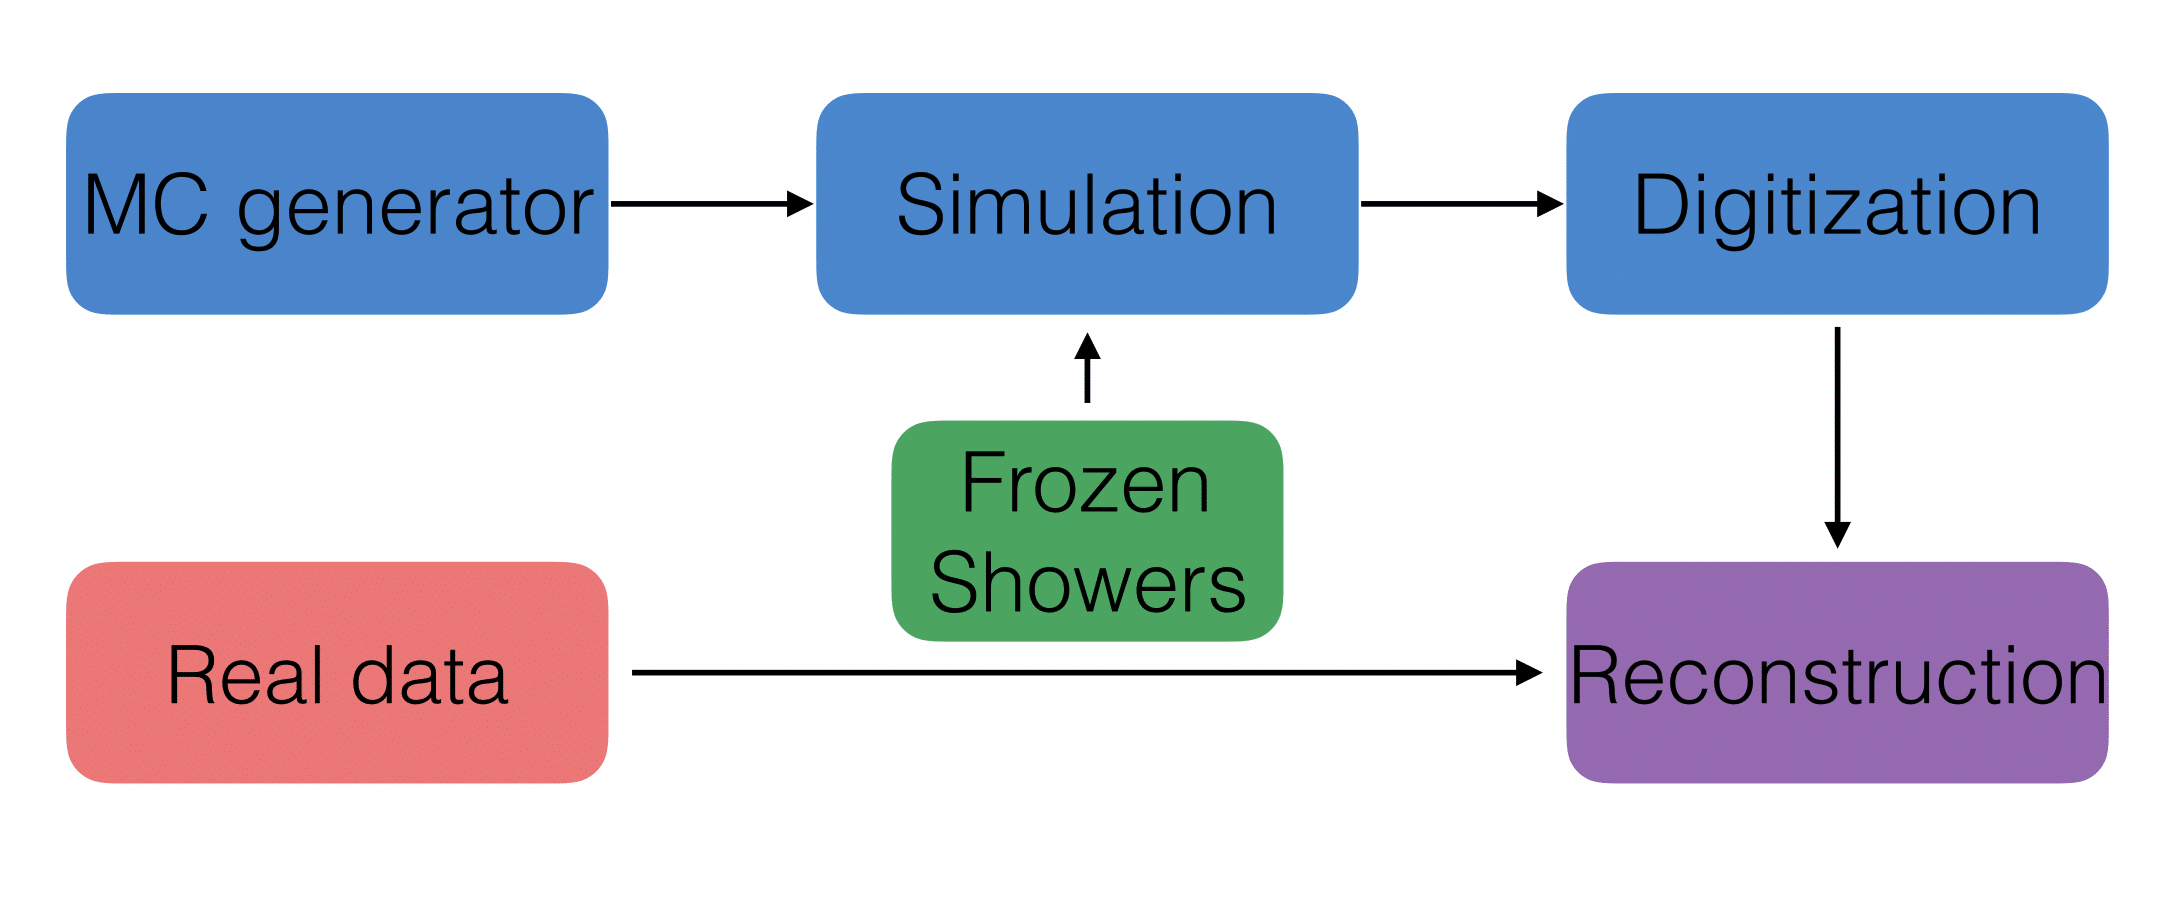
\includegraphics[width=0.6\textwidth]{MC/MCScheme.png}
\caption{Diagram of the \atlas MC simulation chain.}
\label{fig:MC_gen2}}
\end{figure}

Monte Carlo method allows to perform different types of analyses, such as predictions generation for comparisons with data, study the detector or the selection algorithms performance. The \atlas simulation software is integrated into Athena framework used at \atlas experiment \cite{Athena}. Simulation chain is can be divided into four main steps (Fig.~\ref{fig:MC_gen2}):
\begin{description}
\item[Event generation] Simulation of hard interaction, parton evolution and hadronization. This step is independent of the \atlas detector geometry;
\item[Detector simulation] Simulation of energy deposits ("hits") which are produced by final state particles;
\item[Digitalization] Simulation of detector electronics response. This procedure can be divided into two steps: on first inputs to the read out drivers (ROD's) are simulated, on the second the ROD functionality is emulated. Detector noise effects are also simulated on the second step;
\item[Reconstruction] Production of the Analysis Object Data (AOD) files, which contain the information needed for physics analysis. This stage is identical to both data and MC and discussed in details in Chap.~\ref{chap:Rec}.
\end{description}
Additionally, the pile-up effects are added to MC by overlaying the simulation of the hard interaction with the simulation of additional soft inelastic interactions. In the following sections, event generation and simulation will be described in more details.

\section{Event generation}

\begin{figure}[!t]
\begin{center}
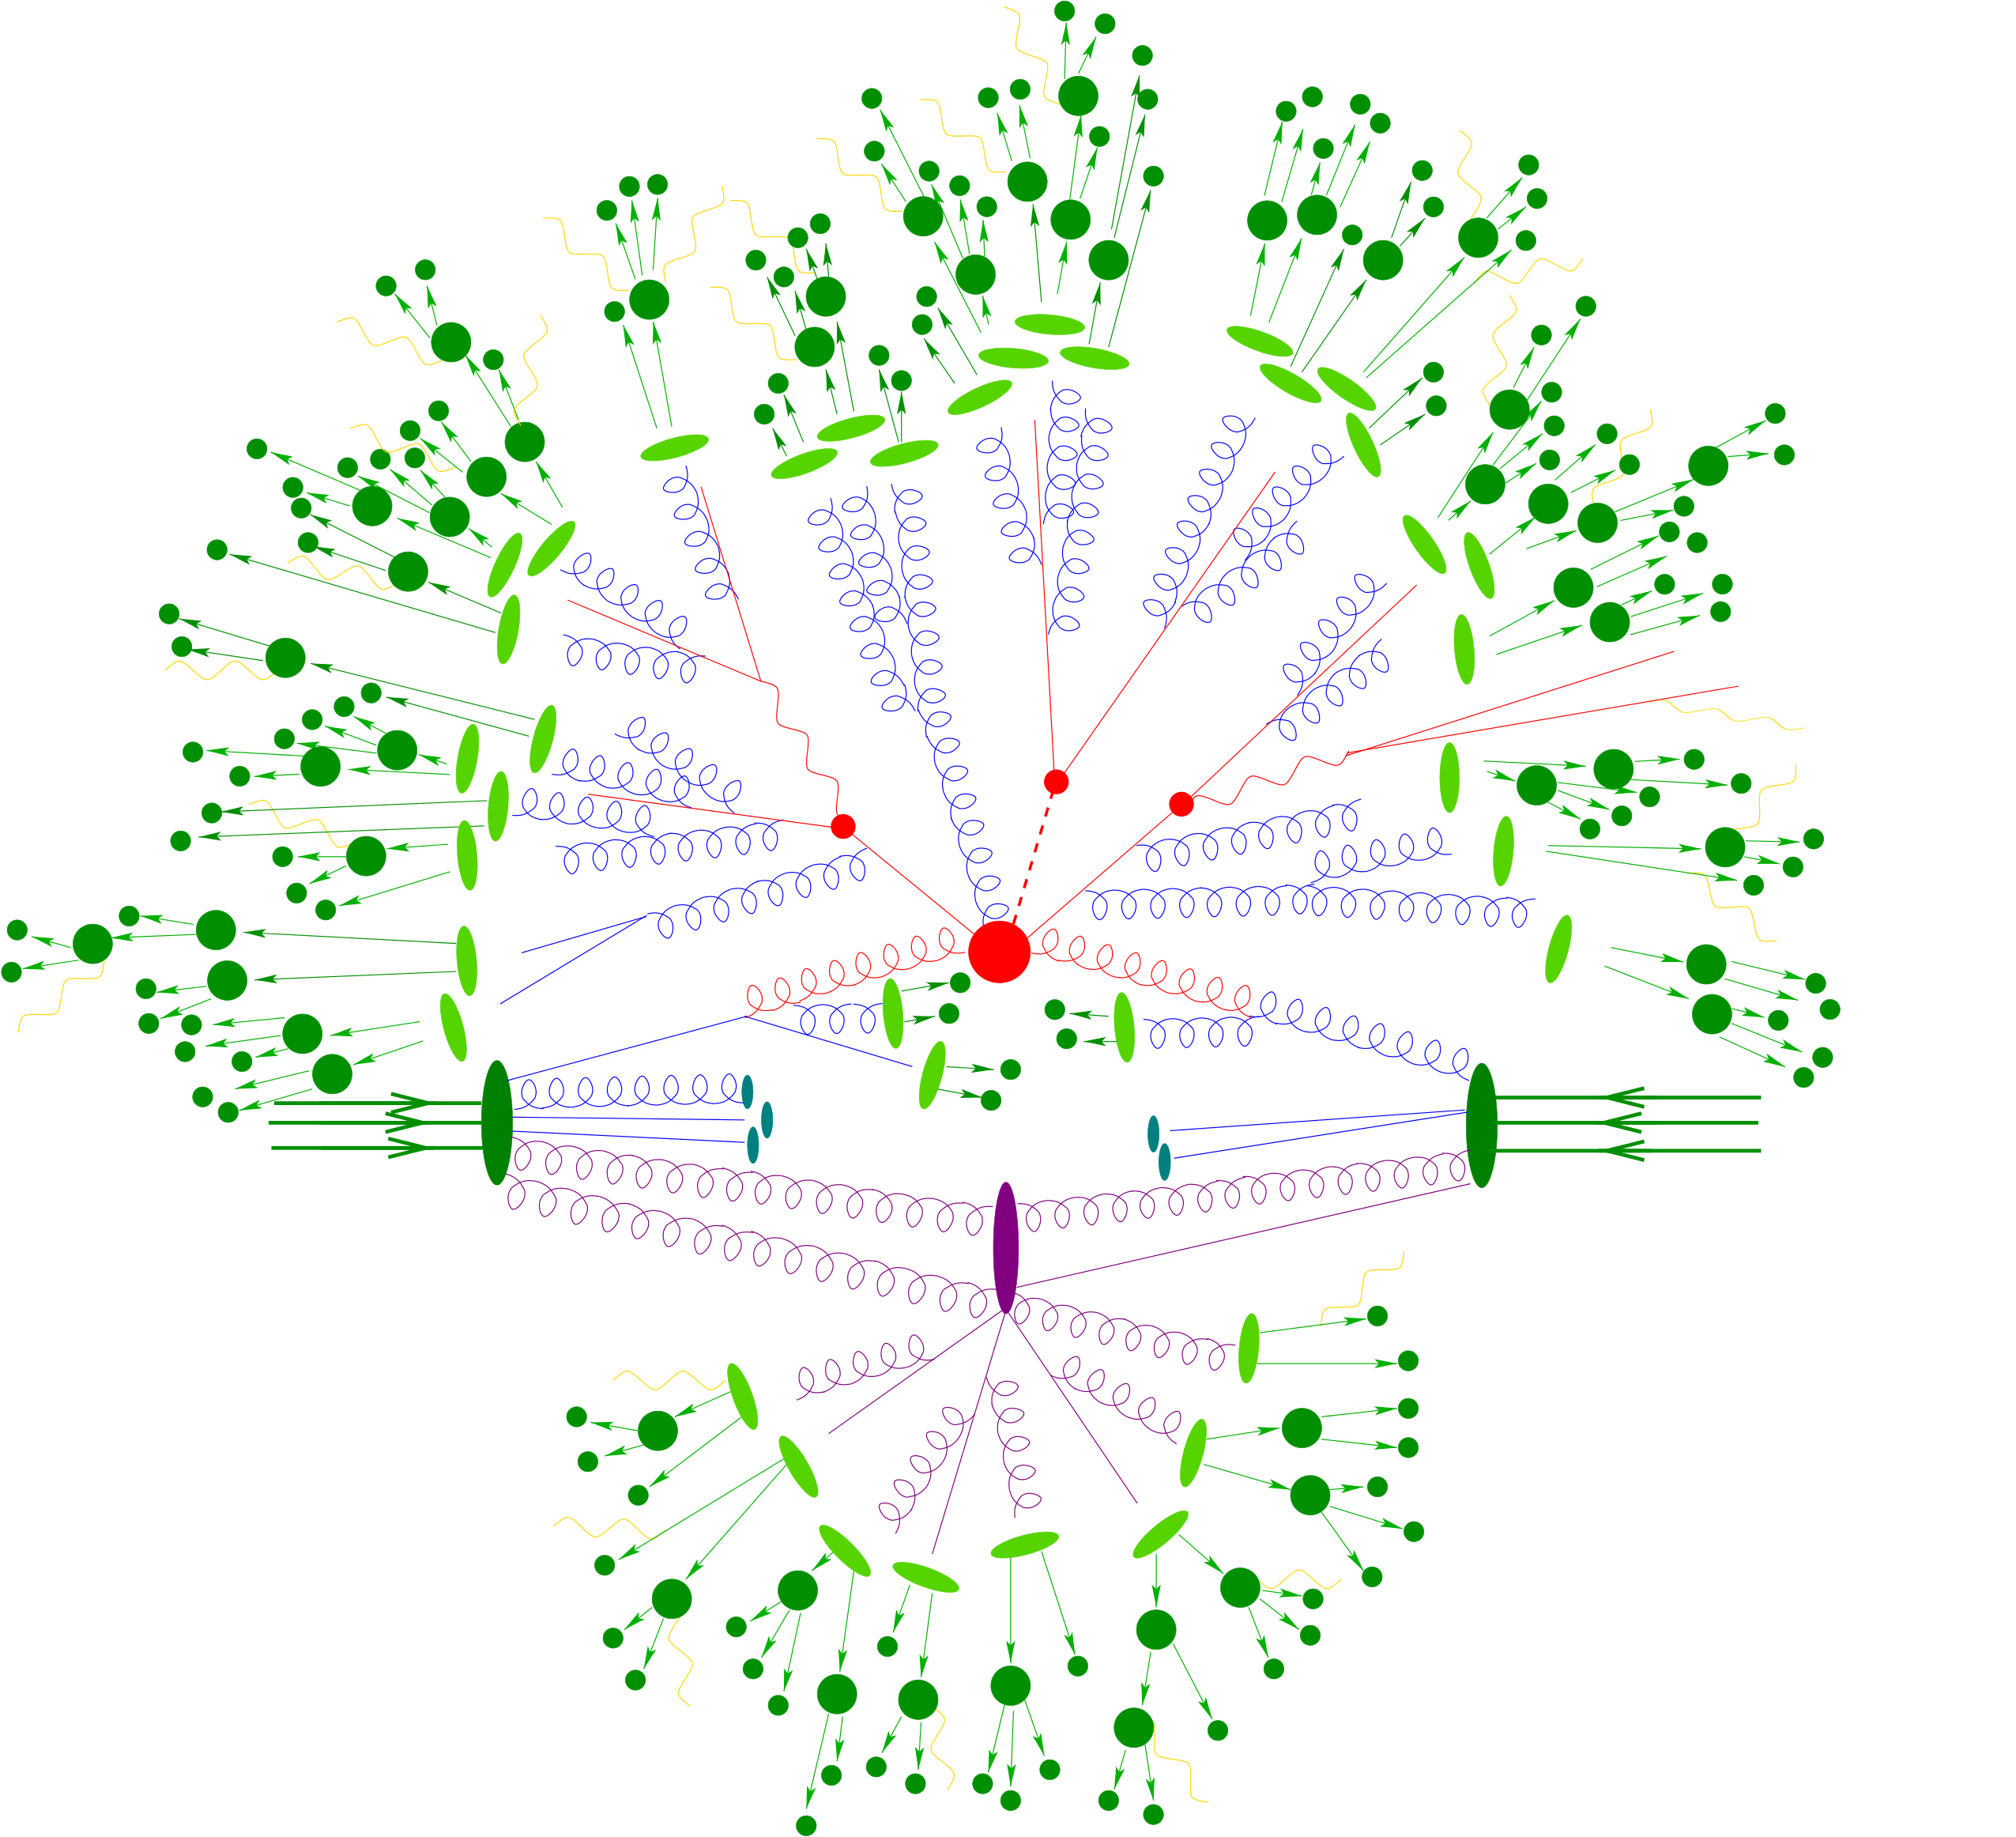
\includegraphics[width=0.5\textwidth]{MC/tth_Event}
\end{center}
\caption{Schematic view of a  top quark pair production associated with a Higgs boson event produced in a pp collision: the hard scattering is shown as a red blob with the solid and dashed lines as the resulting three particles.
Multi-particle interactions are indicated by the violet blob. 
Parton showers are shown with curly lines.
Hadronization is shown in light green, while the final state particles as dark green\cite{MC:ttHSketch}.
}
\label{fig:MC_ttH}
\end{figure}

The main goal of the event generator is to provide a complete picture of the final state: description of the particle types and momenta on  the event-by-event basis. According to the factorization theorem\cite{Factorisation}, the event generation can be divided into four independent stages: 
\begin{description}
\item[Modeling of hard subprocess] The process of interest is simulated from its production channels using the corresponding matrix elements (ME)  at a fixed order of the strong coupling constant. The momenta of the incoming protons in the matrix elements are randomly chosen based on the parton distribution functions (PDF). Most of the generators make simulation at leading (LO) order or next to leading order (NLO) in $\alpha_s$;
\item[Parton showering] Quarks and gluons from hard process can radiate secondary partons, resulting in the production of additional hadrons in the event. This process is calculated as a step-by-step evolution of momentum transfer scales from highest (hard subprocess), to the lowest (around 1 GeV), where the perturbative calculations are not valid. 
There is a possible double counting between showering and hard process simulation can be avoided using different matching approaches. 
\item[Hadronization] Final-state hadrons, which can be detected in an experiment, are formed during hadronization step. This process occurs at large scales, where perturbative calculations are not applicable and usually implemented using different phenomenological models\cite{hep-ph/9912292};
\item[underlying event] In parallel to the main process, collisions of other partons can also occur. This effect is called underlying event. 
\end{description}
Scheme of simulation of a top quark pair production associated with a Higgs boson event is shown in Fig.~\ref{fig:MC_ttH}:

The current analysis uses samples generated with the following generators:
\begin{itemize}[align=left]
\item[Powheg \cite{Powheg}]  is a Monte Carlo generator, which calculates the QCD process at the NLO level \cite{PowhegNLO}. It can be interfaced to other generators (such as Pythia or Herwig) to get higher precision of showering;
\item[Pythia \cite{Pythia6}]  is a general purpose generator for simulating hadron-hadron, hadron-lepton and lepton-lepton collisions. It can model initial and final state showers, hadronization, hadron decays and underlying event. Pythia contains around 240 QCD processes at LO. It uses Lund String model \cite{LundString} to simulate hadronization;
\item[Herwig \cite{Herwig}] is an LO general purpose event generator for simulation of lepton-lepton, hadron-lepton and hadron-hadron collisions. The main difference between Pythia and Herwig is that Herwig uses angular ordering in the parton showers\cite{hep-ph/0612282} and models the hadronization using the cluster fragmentation\cite{Kupco:390985};
\item[Sherpa \cite{Sherpa}]  is an event generator, that uses LO QCD predictions for a hard scattering and features its own implementation of parton shower and hadronization models;
\item[Photos \cite{Photos}]  is a program used to generate QED radiative corrections, that is additionally liked to  multipurpose generators;
\item[Tauola \cite{taluola}] is a generator, used to describe leptonic and semi-leptonic $\tau$-decays, that is additionally liked to  multipurpose generators.
\end{itemize}

\section{Detector simulation}

After event generation step, a dedicated simulation software is used to provide detector response for final state particles. The main method used by \atlas experiment, referred to as a \textit{Full Simulation}, uses of the Geant4\cite{Geant4} libraries. Geant4 is a C++ based toolkit for the simulation of the passage of particles through the matter. It is used in a wide range of experiments in the high energy and nuclear physics.

The Geant4 can simulate complex detector structures with sensitive detector material and corresponding infrastructure. It can also calculate basic properties of composite materials, like radiation and interaction length. Geant4 stores "hits" information  - snapshots of physical interactions. 
In Geant4 events and particles are simulated separately and each particle is moved in steps. The size of each step is chosen to preserve both CPU performance and required precision. 

Interactions of particles with the detector are treated as a set of discrete processes. Geant4 package provides different models for hadronic and electromagnetic interaction processes. It allows choosing a set of the models (called physics list) depending on particular requirements. There are several reference physics lists, that are validated for each new release of Geant4 software. \atlas experiment uses one of these lists.

The simulation of detector response is the most CPU-time consuming part in the \atlas simulation chain. Most of the CERN computing resources are used by a mass MC production, required for each data taking period. Uncertainties of some of Run-I analyses are dominated by available MC statistics. It is possible to improve the CPU usage by tuning physics list or replacing complex magnetic field maps by a parameterization. Additionally, there are long-term developments for multi-threading and vectorization of the code.  The fast and accurate simulation approach is essential. During the simulation largest time is spent on simulation of calorimeters. This is a motivation for the development of a fast calorimetry simulation techniques.  

There are two main methods currently used by \atlas to reduce the time needed for the simulation of the calorimeter response\cite{Lukas:1458503}: 
\begin{itemize}
\item Parameterization of the calorimeter cells response. The spacial energy response is simulated using longitudinal and lateral energy profiles;
\item Frozen Showers. This technique is described in Chap.~\ref{chap:FS}.
\end{itemize}

